\documentclass[border=8pt]{standalone}

\usepackage{pgfplots}
\pgfplotsset{compat=1.18}

% ----------------------------------------------------------
%  Cornell Palette
% ----------------------------------------------------------
\definecolor{CornellRed}   {RGB}{179, 27,  27}
\definecolor{CornellDark}  {RGB}{ 91,  0,   0}
\definecolor{CornellMid}   {RGB}{140, 20,  20}
\definecolor{CornellAccent}{RGB}{220,170,170}
\definecolor{CornellLight} {RGB}{250,238,238}
\definecolor{CornellGray}  {RGB}{ 84, 88,  90}
\definecolor{LoRABlue}     {RGB}{ 60,100,165}
\definecolor{NumGreen}     {RGB}{ 30,120, 60}
\definecolor{BodyBg}       {RGB}{255,255,255}
\definecolor{TableShade}   {RGB}{253,238,238}

\begin{document}
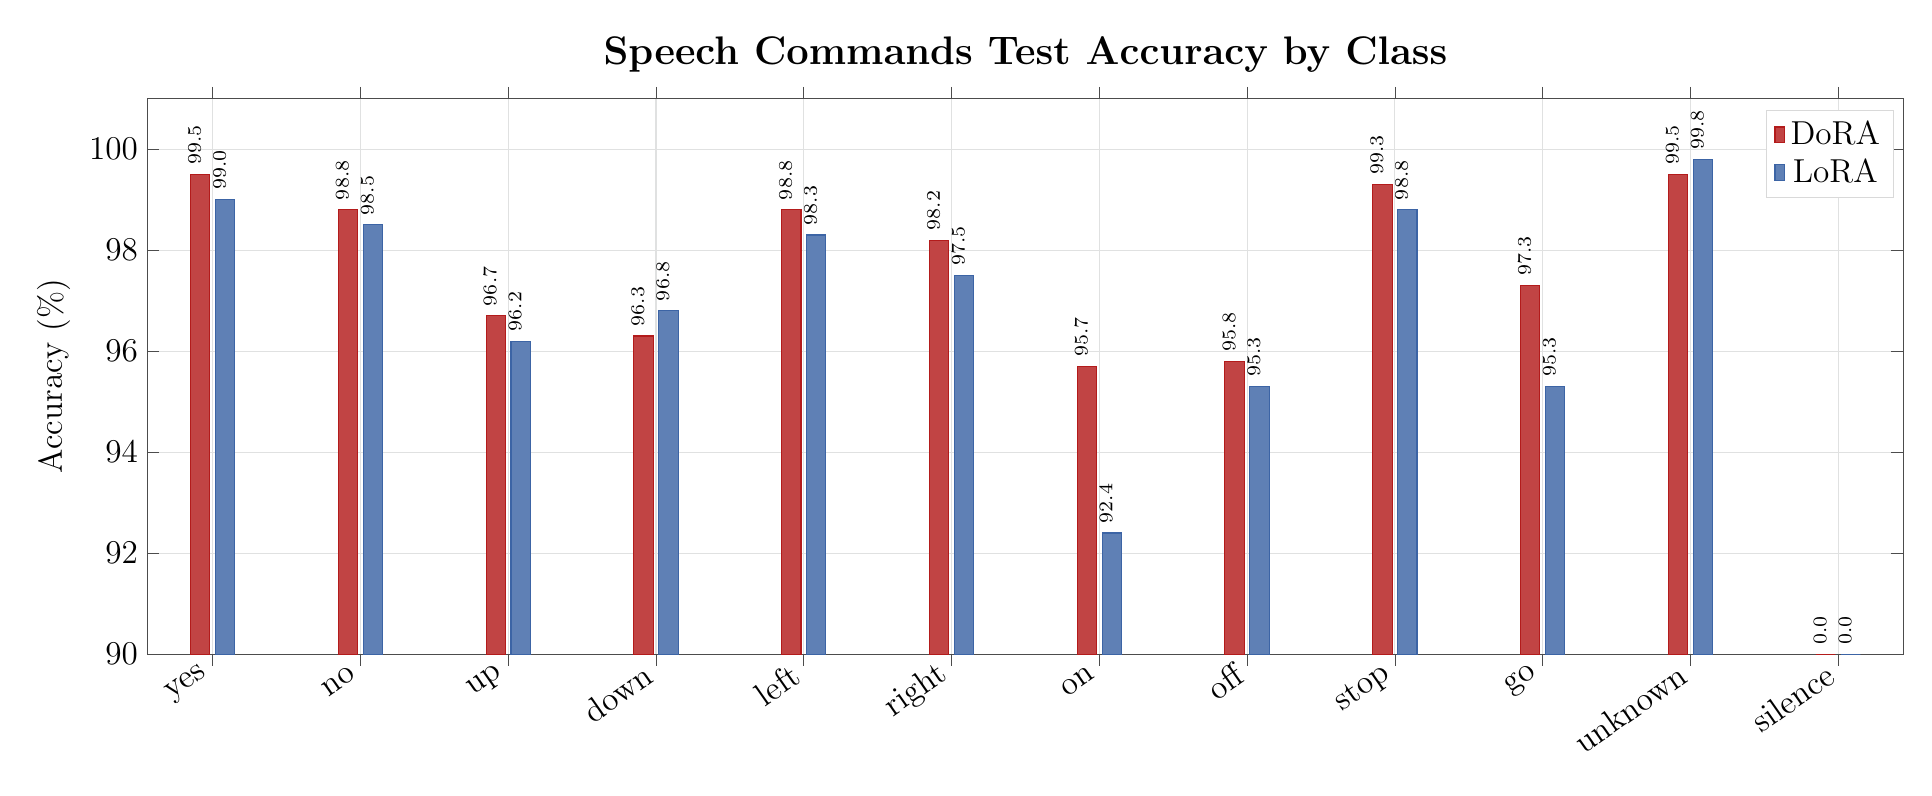
\begin{tikzpicture}
\begin{axis}[
    width=9.4in,
    height=3.4in,
    ybar,
    bar width=7pt,
    title={Speech Commands Test Accuracy by Class},
    title style={font=\bfseries\Large},
    ylabel={Accuracy (\%)},
    label style={font=\large},
    tick label style={font=\large},
    ymin=90,
    ymax=101,
    ytick={90,92,94,96,98,100},
    symbolic x coords={
        yes,
        no,
        up,
        down,
        left,
        right,
        on,
        off,
        stop,
        go,
        unknown,
        silence
    },
    xtick=data,
    xticklabel style={
        rotate=35,
        anchor=east,
        font=\large
    },
    enlarge x limits=0.04,
    grid=major,
    major grid style={draw=CornellGray!18},
    axis line style={draw=black!70},
    tick style={draw=black!70},
    legend style={
        at={(0.995,0.98)},
        anchor=north east,
        draw=black!15,
        fill=BodyBg,
        font=\large
    },
    legend image code/.code={
        \draw[#1] (0cm,-0.1cm) rectangle (0.12cm,0.1cm);
    },
    point meta=explicit symbolic,
    nodes near coords={\pgfplotspointmeta},
    nodes near coords align={vertical},
    every node near coord/.append style={
        font=\scriptsize,
        rotate=90,
        anchor=west,
        yshift=2pt,
        /pgf/number format/fixed,
        /pgf/number format/precision=1
    },
]

\addplot[
    fill=CornellRed!82,
    draw=CornellRed,
] coordinates {
    (yes,99.5) [99.5]
    (no,98.8) [98.8]
    (up,96.7) [96.7]
    (down,96.3) [96.3]
    (left,98.8) [98.8]
    (right,98.2) [98.2]
    (on,95.7) [95.7]
    (off,95.8) [95.8]
    (stop,99.3) [99.3]
    (go,97.3) [97.3]
    (unknown,99.5) [99.5]
    (silence,90.0) [0.0]
};
\addlegendentry{DoRA}

\addplot[
    fill=LoRABlue!82,
    draw=LoRABlue,
] coordinates {
    (yes,99.0) [99.0]
    (no,98.5) [98.5]
    (up,96.2) [96.2]
    (down,96.8) [96.8]
    (left,98.3) [98.3]
    (right,97.5) [97.5]
    (on,92.4) [92.4]
    (off,95.3) [95.3]
    (stop,98.8) [98.8]
    (go,95.3) [95.3]
    (unknown,99.8) [99.8]
    (silence,90.0) [0.0]
};
\addlegendentry{LoRA}

\end{axis}
\end{tikzpicture}
\end{document}
